\documentclass[11pt]{article}
\usepackage[T1]{fontenc}
\usepackage[utf8]{inputenc}
\usepackage{lmodern}
\usepackage[a4paper,margin=1in]{geometry}
\usepackage{amsmath,amssymb,amsthm,mathtools}
\usepackage{microtype}
\usepackage{booktabs}
\usepackage{tabularx}
\usepackage{array}
\usepackage{xcolor}
\usepackage{pgfplots}
\pgfplotsset{compat=1.18}
\usepackage{algorithm}
\usepackage{algpseudocode}
\usepackage[authoryear,round]{natbib}
\usepackage[colorlinks=true,linkcolor=black!70!green,citecolor=black!70!green,urlcolor=black!70!green]{hyperref}
\usepackage[capitalise,noabbrev]{cleveref}
\usepackage{enumitem}
\setlist{itemsep=2pt,topsep=4pt}

\newtheorem{theorem}{Theorem}[section]
\newtheorem{proposition}[theorem]{Proposition}
\newtheorem{lemma}[theorem]{Lemma}
\newtheorem{corollary}[theorem]{Corollary}
\theoremstyle{definition}
\newtheorem{definition}[theorem]{Definition}
\newtheorem{assumption}[theorem]{Assumption}
\newtheorem{example}[theorem]{Example}
\theoremstyle{remark}
\newtheorem{remark}[theorem]{Remark}
\crefname{assumption}{Assumption}{Assumptions}

\newcommand{\E}{\mathbb{E}}
\renewcommand{\P}{\mathbb{P}}
\newcommand{\F}{\mathcal{F}}
\newcommand{\G}{\mathcal{G}}
\newcommand{\KL}{\mathrm{KL}}
\newcommand{\kl}{\mathrm{kl}}
\newcommand{\1}{\mathbf{1}}
\newcommand{\eps}{\varepsilon}
\newcommand{\Kinf}{K_{\inf}}
\newcommand{\status}[1]{{\unskip\nobreak\hfil\penalty50\hskip1em\hbox{}\nobreak\hfill\textit{\small[#1]}\parfillskip=0pt\par}}
\DeclareMathOperator*{\argmax}{arg\,max}

\definecolor{cpine}{HTML}{1D4A3A}
\definecolor{cverm}{HTML}{A63A1D}
\definecolor{cbrass}{HTML}{7A5C20}
\definecolor{csky}{HTML}{4F6FB4}
\definecolor{cgrey}{HTML}{9C9F98}

\title{Verifiers That Do Not Trust the Agent:\\ Anytime-Valid Release Gates and Hacking Bounds\\ for AI Agents That Move Money}
\author{Dhruv Hegde\\ {\normalsize Scruple}\\ {\normalsize\texttt{dhegde@umich.edu}}}
\date{Preprint, November 2026}

\begin{document}
\maketitle

\begin{abstract}
AI agents that handle card disputes move money: they decide when to refund, when to fight and with which evidence. Changes to them are usually judged by win rates and by the agent's own reports, and both can be gamed. We describe a release gate whose verifiers never credit the agent's claims: cost is recomputed from double-entry ledger postings, and every action is checked against a hash-chained trace written by the environment. Its statistics are anytime-valid. We prove that if each hacked case is caught with conditional probability at least $\rho$, whatever the agent knows, an accepted change carries a proxy-over-ledger gap $\Gamma\ge\gamma$ with probability at most $(1-\rho)^{\lceil n\gamma/\eps\rceil}$; we give $\rho$ for audits that leak, the audit rate at which hacking stops paying when the verifier errs both ways, and what the composed promote decision guarantees. On a frozen synthetic benchmark of 10{,}000 disputes, one of four pre-registered experiments passed (narrowly), two failed their primary hypothesis and one found no effect; we report why. An optimiser on a naive proxy learned forgery that the simulated ledger rated cheaper. Six learner types used no exploit when trained on the scorecard and found exploits on the proxy. Real Claude models exposed three verifier false positives.
\end{abstract}

\paragraph{Data and labels.} Numbers marked \emph{synthetic} come from the scruple simulator; numbers marked \emph{real} come from public CFPB complaint data or from real model behaviour. No number describes a real merchant, bank or card network. Each result is labelled \emph{standard} (known, applied here), \emph{adaptation} (a small variant of a known result) or \emph{candidate novel} (not found stated this way in a short search; a full literature review is still required). Code, data and every result file: \url{https://github.com/thedhruvhegde/scruple}, directory \texttt{engine/}.

\section{Introduction}

Card disputes are a good test bed for agents that move money. Every case ends in postings to a ledger: a refund, a chargeback, a fee, a representment won or lost. The rules are public (Regulation~E, 12 CFR 1005.11, for debit cards; Regulation~Z, 12 CFR 1026.13, for credit cards), and the incentives to cheat are concrete. An agent judged on its win rate can fight claims it should concede, cite documents it never opened, upload documents that never existed, or simply report a win.

The usual guard for an agent change is an offline evaluation: replay the new agent on held-out cases, compare a metric, ship if it improves. That guard fails in three ways that we measure.
\begin{enumerate}
\item \textbf{The metric trusts the agent.} In our experiment E2 a seeded hill climb on a ``wins plus self-reported wins'' proxy learned two exploits (fabricated documents and false win claims) in three moves.
\item \textbf{The statistics do not survive how they are used.} Re-running a $z$-test every 10 cases at the null boundary rejects 14.7\% to 34.3\% of the time at a nominal 5\% (synthetic). A regression of 0.35 cap units in a case type that is 1\% of traffic, with the rest improving, is flagged by a pooled valid test 0.6\% of the time.
\item \textbf{Nobody states what the release decision guarantees.} A gate mixes deterministic checks, soft scores and tests; which error does the combination control?
\end{enumerate}

\paragraph{Contributions.}
\begin{itemize}
\item A verifier design anchored to the ledger and to an environment-written trace, with an attack for every check (\cref{sec:verifiers}), and a record of what broke: an engine bug found through verifier false alarms, false positives found by real models, and three exploits closed.
\item Anytime-valid paired and stratified tests with complete proofs (\cref{sec:sequential,sec:stratified}), sample-size planning with a matching lower bound (\cref{sec:planning}), and variance-adaptive betting with a sample-size floor computed from observed data (\cref{sec:betting}).
\item A composition theorem for the release decision (\cref{sec:composition}) and its asymmetric-cost refinement (\cref{sec:decision}).
\item Hacking-gap bounds for adaptive agents with leaky audits and an imperfect verifier, and the minimal audit rate that removes the incentive to hack (\cref{sec:hacking}).
\item Four pre-registered experiments, reported whichever way they fell: planted regressions (E1, pass), an optimiser on a naive proxy (E2, fails H2), a variance-reduced gate (E3, fails H1) and a win-rate incentive for real models (E4, H1 not supported) (\cref{sec:experiments}).
\item A comparison of six learner types under the scorecard and under the naive proxy; 64 dispute scenarios grounded in real CFPB complaints, and a timeliness analysis of 164{,}821 real complaints.
\end{itemize}

\section{Setting and notation}\label{sec:setting}

\begin{definition}[Episode and record]
A dispute episode starts from a seeded case: a card transaction, a reason code, a cardholder claim with a hidden truth (valid or not), documents the merchant does or does not hold, and network deadlines. The agent acts through tools (read the case, list and read evidence, request information, read the ledger, refund, represent, accept, wait, upload evidence). The environment writes every call and every state change to an append-only trace whose events are hashed into a chain with a recorded head. Money is double-entry, in USD minor units. The \emph{record} of an episode is the trace, the final journal, the documents as generated and at close, the case with its hidden truth, and the agent's self-report.
\end{definition}

\begin{definition}[Paired difference]
A candidate policy $C$ is compared with the current policy $B$ on the same held-out cases and the same issuer draws. Case $i$ gives losses $B_i, C_i$ (merchant cost from the journal). Before outcomes are seen the operator declares a cap $c>0$, and
\begin{equation}\label{eq:x}
X_i = \frac{C_i - B_i}{c} \in [-1,1], \qquad \mu_i = \E[X_i \mid \F_{i-1}],
\end{equation}
where $\F_{i-1}$ is everything observed before case $i$. Positive $X_i$ means the candidate is worse.
\end{definition}

\begin{assumption}[Cap]\label{ass:cap}
$|C_i - B_i|\le c$ for every case. A violation is an error; it is never clipped silently.
\end{assumption}

\begin{assumption}[Predictable bets]\label{ass:pred}
Every bet $\lambda_i$ used for case $i$ is $\F_{i-1}$-measurable.
\end{assumption}

The gate decides \emph{promote}, \emph{hold} or \emph{block}. The error that costs money is promoting a harmful change; the error that costs adoption is blocking a good one.

\paragraph{Benchmark.} Benchmark v1 is 10{,}000 synthetic dispute cases from a sealed held-out seed namespace; only a manifest of commitments is public (content hash \texttt{1286baf3\ldots2cb13f91}). Family mix: buyer's remorse 1{,}977; cardholder mistake 577; friendly fraud 2{,}791; merchant error 625; service failure 1{,}840; true fraud 2{,}190; 4{,}655 claims are valid. Reference policies (synthetic): the \emph{evidence} policy (represent when the required evidence exists, else concede) costs \$82.82 per case (95\% interval 80.72 to 84.91) and fails a hard check on 19 of 10{,}000 cases; always-accept costs \$127.46; an oracle that reads the hidden truth costs \$86.67, more than the evidence policy, because knowing a claim is invalid does not win it without documents.

\section{Verifier design: anchoring to the ledger and the trace}\label{sec:verifiers}

The design principle is that nothing the agent says earns credit. Self-reports are \emph{checked}, never \emph{scored}: a self-report can only lose points. Scores compose as
\begin{equation}\label{eq:reward}
\text{gate} = \textstyle\bigwedge_{h}\text{hard}_h,\qquad \text{quality} = \sum_j w_j s_j \big/ \sum_j w_j,\qquad \text{reward} = \text{gate}\times\text{quality},
\end{equation}
so a hard failure zeroes the reward and ten perfect soft scores cannot outvote one violation. \Cref{tab:checks} lists the checks and, for each, an attack that fools a naive metric and is stopped by the check.

\begin{table}[t]
\centering\small
\caption{Checks, what they read, and the attack each stops. Synthetic, 300 seeds per attack.}\label{tab:checks}
\begin{tabularx}{\linewidth}{@{}l>{\raggedright\arraybackslash}Xl>{\raggedright\arraybackslash}X@{}}
\toprule
check & reads & kind & attack stopped (naive metric fooled) \\
\midrule
INV-01 ledger invariants & trace postings, after every action & hard & double credit then moot \\
INV-05 record integrity & hash chain and head & hard & outcome rewrite (correct rate 1.0) \\
PROC-01 process & trace order & hard & summary response (half the calls) \\
EVD-01 provenance & generator truth, content hashes & hard & fabrication (win rate 0.044 to 0.85) \\
DL-01 deadlines & env-recorded network calendar & hard & stall on pending information \\
SR-01 self-report & claims parsed into predicates on the record & hard & claimed, not done \\
SCOPE-01 scope & protected reads, tool and argument scope & hard & ground-truth peeking \\
CON-01, CAL-01, SR-03 & batch statistics & hard & segment skimming, flat confidence \\
CF-01 counterfactual & replay under baseline, same draws & soft & refund to win \\
OUT-01 fair outcome & hidden truth & soft & unfair wins (\cref{sec:episodes}) \\
\bottomrule
\end{tabularx}
\end{table}

On 300 synthetic seeds the exploit run reports, by row: caught 28, blocked 5 (the environment refuses the move), partial 1, not caught 1, not modelled 7. ``Caught'' means the naive metric rates the exploit at least as well as the honest policy, the expected check fires on at least 90\% of exercised episodes, and the reward falls. The partial case is ``escalate everything'' (94 of 125 exercised episodes caught; on the rest it wins a valid claim cheaply and only the soft OUT-01 notices); the one not caught is ``memorised outcomes'' (0 of 30). Mutation testing of the 18 verifier modules (2{,}173 mutants) gave a mutation score of 63.8\%, 64.7\% after 15 targeted tests.

\section{Anytime-valid paired test}\label{sec:sequential}

We first record the two probabilistic tools every later proof uses.

\begin{lemma}[Ville's inequality]\label{lem:ville}
Let $(K_t)_{t\ge0}$ be a non-negative supermartingale with $K_0=1$. Then for every $a>0$, $\P(\exists t: K_t\ge a)\le 1/a$, and for every stopping time $\tau$ (possibly infinite, with $K_\infty=\liminf_t K_t$), $\E[K_\tau]\le 1$.
\status{standard; \citealp{ville1939}}
\end{lemma}
\begin{proof}
Let $\sigma=\inf\{t:K_t\ge a\}$. For fixed $T$, $\sigma\wedge T$ is a bounded stopping time, so by optional stopping for supermartingales \citep[Ch.~4]{durrett2019} $\E[K_{\sigma\wedge T}]\le K_0=1$. Since $K\ge0$ and $K_{\sigma\wedge T}\ge a$ on $\{\sigma\le T\}$, $a\,\P(\sigma\le T)\le 1$. Let $T\to\infty$: $\P(\sigma<\infty)\le 1/a$. For the second claim, $K_{\tau\wedge T}\to K_\tau$ on $\{\tau<\infty\}$ and $\liminf_T K_{\tau\wedge T}=\liminf_t K_t = K_\infty$ on $\{\tau=\infty\}$; Fatou's lemma gives $\E[K_\tau]\le\liminf_T\E[K_{\tau\wedge T}]\le 1$.
\end{proof}

\begin{lemma}[Data processing for KL]\label{lem:dp}
Let $\kl(p\|q)=p\log\tfrac pq+(1-p)\log\tfrac{1-p}{1-q}$. For laws $P,Q$ and any event $A$, $\KL(P\|Q)\ge \kl(P(A)\|Q(A))$. If $P(A)\ge 1-\beta > \alpha\ge Q(A)$, then $\kl(P(A)\|Q(A))\ge\kl(1-\beta\|\alpha)$.
\status{standard; \citealp{cover2006}}
\end{lemma}
\begin{proof}
The first inequality is the data-processing inequality applied to the map $\omega\mapsto\1_A(\omega)$. For the second, $\partial_p\kl(p\|q)=\log\frac{p(1-q)}{q(1-p)}\ge0$ for $p\ge q$ and $\partial_q\kl(p\|q)=\frac{q-p}{q(1-q)}\le 0$ for $q\le p$; so increasing $p$ from $1-\beta$ and decreasing $q$ from $\alpha$ only increases $\kl$.
\end{proof}

\begin{proposition}[Betting e-process]\label{prop:betting}
Fix $m\in(-1,1)$ and a side $s\in\{+1,-1\}$ ($s=+1$: regression, $H_0:\mu_i\le m$ for all $i$; $s=-1$: certification, $H_0:\mu_i\ge m$ for all $i$). Let $Y_i=s(X_i-m)$ and predictable bets $0\le\lambda_i\le b/(1+sm)$ with $b<1$. Then
\begin{equation}\label{eq:wealth}
K_t=\prod_{i\le t}(1+\lambda_iY_i)
\end{equation}
satisfies, under $H_0$, $\P(\exists t:K_t\ge1/\alpha)\le\alpha$, and $\E[K_\tau]\le1$ for every stopping time $\tau$.
\status{standard; \citealp{ramdas2023,waudbysmith2023}}
\end{proposition}
\begin{proof}
Since $X_i\in[-1,1]$, $Y_i\ge -(1+sm)$, so $1+\lambda_iY_i\ge 1-b>0$ and $K_t>0$. Under $H_0$, $s(\mu_i-m)\le 0$; as $\lambda_i\ge0$ is $\F_{i-1}$-measurable, $\E[1+\lambda_iY_i\mid\F_{i-1}]=1+\lambda_i s(\mu_i-m)\le1$. Hence $K$ is a non-negative supermartingale with $K_0=1$, and \cref{lem:ville} with $a=1/\alpha$ gives both claims.
\end{proof}

\begin{algorithm}[t]
\caption{Paired regression or certification test (default bet: aGRAPA)}\label{alg:betting}
\begin{algorithmic}[1]
\Require cap $c$, null mean $m$, side $s$, level $\alpha$, max bet $b<1$, prior second moment $v_0=1/4$
\State $\log K\gets0$, $S_1\gets0$, $S_2\gets0$, $n\gets0$
\For{each case $i$ as it resolves}
  \State $\lambda\gets \min\{\max\{(S_1/(n+1))/((v_0+S_2)/(n+1)),0\},\ b/(1+sm)\}$ \Comment{uses past data only}
  \State $Y\gets s((C_i-B_i)/c-m)$; \quad $\log K\gets\log K+\log(1+\lambda Y)$
  \State $S_1\gets S_1+Y$, $S_2\gets S_2+Y^2$, $n\gets n+1$
  \If{$\log K\ge\log(1/\alpha)$} \Return reject $H_0$ at case $n$ \EndIf
\EndFor
\State \Return do not reject
\end{algorithmic}
\end{algorithm}

The aGRAPA bet of \cref{alg:betting} maximises $\lambda\E Y-\lambda^2\E Y^2/2$, the second-order expansion of the growth rate $\E\log(1+\lambda Y)$ \citep{kelly1956,waudbysmith2023}. It affects power only, never validity.

\begin{proposition}[Exact-interval confidence sequence]\label{prop:cs}
Let $X_i$ be i.i.d.\ with mean $\mu$, and let $\lambda_i\in[0,b]$, $b<1/2$, be predictable and not depend on the candidate mean $m$. Set $K^+_t(m)=\prod_{i\le t}(1+\lambda_i(X_i-m))$, $K^-_t(m)=\prod_{i\le t}(1+\lambda_i(m-X_i))$ and
\[
C_t=\{m\in[-1,1]: K^+_t(m)<2/\alpha\text{ and }K^-_t(m)<2/\alpha\}.
\]
Then each $C_t$ is an interval, $\P(\forall t:\mu\in C_t)\ge1-\alpha$, and the same holds for the running intersection $\bigcap_{s\le t}C_s$.
\status{adaptation of \citealp{waudbysmith2023}}
\end{proposition}
\begin{proof}
For $m\in[-1,1]$ every factor $1+\lambda_i(X_i-m)\ge 1-2b>0$ and is non-increasing in $m$; a product of positive non-increasing functions is non-increasing, so $\{m:K^+_t(m)\ge2/\alpha\}$ is an initial segment of $[-1,1]$. Symmetrically $\{m:K^-_t(m)\ge2/\alpha\}$ is a final segment, so $C_t$ is an interval. At $m=\mu$, $\E[1+\lambda_i(X_i-\mu)\mid\F_{i-1}]=1$, so $K^\pm_t(\mu)$ are non-negative martingales with initial value 1; by \cref{lem:ville} each exceeds $2/\alpha$ at some time with probability at most $\alpha/2$, and by a union bound $\mu\in C_t$ for all $t$ with probability at least $1-\alpha$. On that event $\mu$ lies in every $C_s$ and so in their intersection.
\end{proof}

\paragraph{Evidence (synthetic).} Nulls at the boundary $\mu=m=0$, four null shapes, seven stopping rules applied to the same 2{,}000 paths of 2{,}000 cases (including ``stop when it looks bad''): the worst rejection rate of the betting test was $0.027$ at $\alpha=0.05$. A one-sided $z$-test re-run every 10 cases rejected $0.147$ to $0.343$ of the time (\cref{fig:peek}). Power (ternary data, 10\% of cases changed) is in \cref{fig:power}.

\begin{figure}[t]
\centering
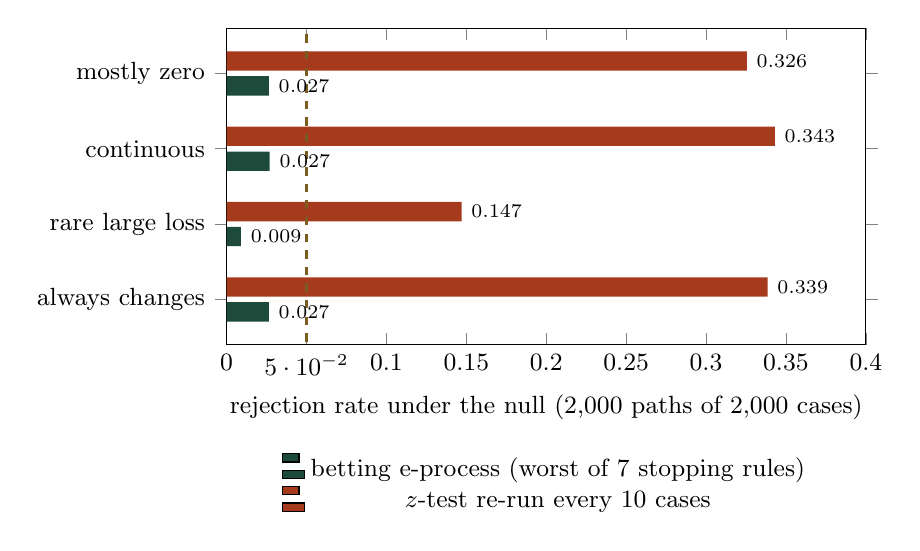
\begin{tikzpicture}
\begin{axis}[xbar, width=0.8\linewidth, height=5.6cm, bar width=7pt, xmin=0, xmax=0.4,
  symbolic y coords={always changes,rare large loss,continuous,mostly zero}, ytick=data,
  xlabel={rejection rate under the null (2{,}000 paths of 2{,}000 cases)}, enlarge y limits=0.2,
  legend style={at={(0.5,-0.32)},anchor=north,font=\small,draw=none,legend columns=1}, nodes near coords, nodes near coords style={font=\scriptsize},
  every node near coord/.append style={/pgf/number format/fixed,/pgf/number format/precision=3},
  tick label style={font=\small}, label style={font=\small}]
\addplot[fill=cpine,draw=none] coordinates {(0.0265,mostly zero) (0.0270,continuous) (0.0090,rare large loss) (0.0265,always changes)};
\addplot[fill=cverm,draw=none] coordinates {(0.3255,mostly zero) (0.3430,continuous) (0.1470,rare large loss) (0.3385,always changes)};
\draw[dashed,cbrass,thick] (axis cs:0.05,{[normalized]-1}) -- (axis cs:0.05,{[normalized]4});
\legend{betting e-process (worst of 7 stopping rules), $z$-test re-run every 10 cases}
\end{axis}
\end{tikzpicture}
\caption{Continuous monitoring at the null boundary, $\alpha=0.05$ (dashed). Synthetic; \texttt{scripts/math\_sequential.py}.}\label{fig:peek}
\end{figure}

\begin{figure}[t]
\centering
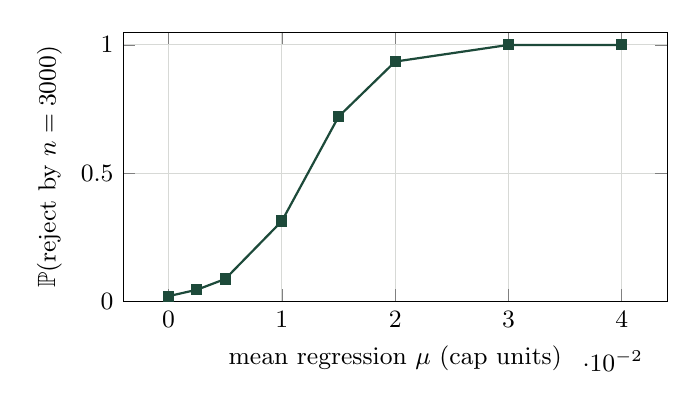
\begin{tikzpicture}
\begin{axis}[width=0.7\linewidth, height=5cm, xlabel={mean regression $\mu$ (cap units)}, ylabel={$\P(\text{reject by }n=3000)$},
  ymin=0, ymax=1.05, grid=major, grid style={cgrey!40}, tick label style={font=\small}, label style={font=\small},
  xticklabel style={/pgf/number format/fixed}]
\addplot[cpine,thick,mark=square*,mark size=1.6pt] coordinates {(0,0.020) (0.0025,0.045) (0.005,0.087) (0.01,0.313) (0.015,0.720) (0.02,0.935) (0.03,1.0) (0.04,1.0)};
\end{axis}
\end{tikzpicture}
\caption{Power of the regression test (aGRAPA), ternary data with 10\% of cases changed by $\pm0.8$, 1{,}000 runs per point. Synthetic.}\label{fig:power}
\end{figure}

\section{Stratified guarantees for rare case types}\label{sec:stratified}

Cases arrive in one stream; each carries a type $k\in\{1,\dots,K\}$ (dispute family) observed before its outcome. For each type, $H_{0,k}:\E[X\mid\text{past},\text{type}=k]\le m_k$, tested by an e-process $E_k$ that updates only on type-$k$ cases.

\begin{lemma}[Stratum e-processes on a shared stream]\label{lem:stratum}
Under $H_{0,k}$, $E_k$ is a non-negative supermartingale for the global filtration, so $\P(\sup_tE_{k,t}\ge a)\le1/a$ and $\E[E_{k,\tau}]\le1$ for every global stopping time $\tau$.
\status{adaptation}
\end{lemma}
\begin{proof}
Let $\F'_{t-1}$ be the global past together with the type of case $t$. If case $t$ has type $k$, the factor is $1+\lambda Y$ with $\lambda$ $\F_{t-1}$-measurable and $\E[1+\lambda Y\mid\F'_{t-1}]\le1$ by the argument of \cref{prop:betting} applied conditionally on the type; otherwise the factor is $1$. Taking conditional expectations given $\F_{t-1}$ preserves the inequality, and \cref{lem:ville} finishes.
\end{proof}

\begin{proposition}[Time-uniform weighted e-Bonferroni]\label{prop:ebonf}
Let $w_k\ge0$ with $\sum_kw_k=K$. Flag type $k$ the first time $E_{k,t}\ge K/(\alpha w_k)$ (never if $w_k=0$). Then $\P(\text{some true null is ever flagged})\le\alpha$, under any dependence between types.
\status{standard}
\end{proposition}
\begin{proof}
By \cref{lem:stratum} with $a=K/(\alpha w_k)$ and a union bound over the set $I_0$ of true nulls, the probability is at most $\sum_{k\in I_0}\alpha w_k/K\le\alpha$.
\end{proof}

\begin{proposition}[Closed testing with mean e-values]\label{prop:closed}
At a stopping time $\tau$, reject $H_{0,k}$ iff $\frac{1}{|S|}\sum_{j\in S}E_{j,\tau}\ge1/\alpha$ for every $S\ni k$. Then the family-wise error is at most $\alpha$; every hypothesis rejected by unweighted e-Bonferroni at level $\alpha$ is rejected; and for each size $s$ the minimum over $|S|=s$, $S\ni k$, is attained by $k$ together with the $s-1$ smallest other e-values.
\status{standard; \citealp{marcus1976,vovkwang2021}}
\end{proposition}
\begin{proof}
Let $I_0$ be the true nulls. The mean $\bar E_{I_0}=\frac1{|I_0|}\sum_{j\in I_0}E_{j,\tau}$ has $\E\bar E_{I_0}\le1$ by \cref{lem:stratum}, so $\P(\bar E_{I_0}\ge1/\alpha)\le\alpha$ by Markov's inequality. A false rejection of some $k\in I_0$ requires the condition for $S=I_0\ni k$, i.e.\ the event above. If $E_k\ge K/\alpha$ then for every $S\ni k$, $\frac1{|S|}\sum_{S}E_j\ge E_k/|S|\ge E_k/K\ge1/\alpha$. For fixed size, the sum over $S$ with $k\in S$ is $E_k$ plus a sum of $s-1$ others, minimised by the smallest ones.
\end{proof}

\begin{proposition}[Weighted e-BH]\label{prop:ebh}
At a stopping time, with $e'_k=w_kE_{k,\tau}$, reject the $r$ largest $e'_k$, where $r$ is the largest $j$ with $e'_{(j)}\ge K/(\alpha j)$. Then $\mathrm{FDR}\le\alpha\sum_{k\in I_0}w_k/K\le\alpha$ under any dependence.
\status{standard; \citealp{wangramdas2022}}
\end{proposition}
\begin{proof}
With $R$ rejections, every rejected $k$ satisfies $e'_k\ge K/(\alpha R)$, so $\1\{k\text{ rejected}\}/\max(R,1)\le\alpha e'_k/K$. Summing over $k\in I_0$ and taking expectations, $\mathrm{FDR}\le\frac\alpha K\sum_{k\in I_0}w_k\E[E_{k,\tau}]\le\frac\alpha K\sum_{k\in I_0}w_k$.
\end{proof}

\begin{remark}
\Cref{prop:closed,prop:ebh} hold at one stopping time; ``reject whenever e-BH has ever rejected'' during monitoring is not covered. The gate uses \cref{prop:ebonf} while monitoring.
\end{remark}

\paragraph{Evidence (synthetic).} Eight types with frequencies $(0.30,0.20,0.15,0.12,0.10,0.08,0.04,0.01)$; the rare type regresses by $+0.35$ cap units while every other type improves by $0.01$, so the pooled mean improves ($-0.0064$). Over 500 runs of 8{,}000 cases a pooled anytime test flagged a regression $0.006$ of the time; stratified e-Bonferroni flagged the rare type $1.000$ of the time. At the null boundary the old zero-tolerance ``no slice mean may get worse'' check false-blocked $0.73$ to $0.996$ of the time, the stratified procedures at most $0.03$.

\section{Planning and the cap tax}\label{sec:planning}

Normalise $m=t_k/c_k$, $d=\Delta_k/c_k$, $\sigma=\sigma_k/c_k$; let $Y=X-m$ with $\E Y=d$, $M_2=\E Y^2=\sigma^2+d^2$, constant bet $\lambda$ and $a=\lambda(1+m)<1$.

\begin{lemma}[Growth bound]\label{lem:growth}
For $a\in[0,1)$ and $x\ge-a$, $\log(1+x)\ge x-\frac{x^2}{2(1-a)}$. Hence $g(\lambda):=\E\log(1+\lambda Y)\ge\lambda d-\frac{\lambda^2M_2}{2(1-a)}$.
\status{adaptation}
\end{lemma}
\begin{proof}
Let $f(x)=\log(1+x)-x+\frac{x^2}{2(1-a)}$. Then $f(0)=0$ and $f'(x)=x\big(\frac1{1-a}-\frac1{1+x}\big)$. For $x\in[-a,0]$, $1+x\ge1-a$ so the bracket is $\ge0$ and $f'\le0$; for $x\ge0$ both factors are $\ge0$. So $f$ is minimised at $0$ and $f\ge0$. Apply with $x=\lambda Y\ge-\lambda(1+m)=-a$ and take expectations.
\end{proof}

\begin{proposition}[Sufficient stratum sample size]\label{prop:samplesize}
Let $Z=\log(1+\lambda Y)$, $v=\lambda^2M_2/(1-a)^2$, $b=\lambda d-\log(1-a)$, $l=\log(1/\beta)$ and $\eps(n)=lb/3+\sqrt{(lb/3)^2+2lnv}$. For i.i.d.\ observations, the constant-bet e-test at level $\alpha_k$ rejects by $n$ observations with probability at least $1-\beta$ whenever
\begin{equation}\label{eq:plan}
n\,g(\lambda)-\eps(n)\ge\log(1/\alpha_k).
\end{equation}
If additionally the type count is $n_k\sim\mathrm{Binomial}(N,\pi_k)$, independent of the type-$k$ outcomes, and $\P(n_k\ge n)\ge1-\gamma$, the power with $N$ total cases is at least $(1-\beta)(1-\gamma)$.
\status{adaptation}
\end{proposition}
\begin{proof}
For $x\ge-a$, $|\log(1+x)|\le|x|/(1-a)$: for $x\ge0$, $\log(1+x)\le x$; for $x\in[-a,0)$, $-\log(1+x)\le -x/(1+x)\le|x|/(1-a)$. Hence $\mathrm{Var}Z\le\E Z^2\le v$. By Jensen, $\E Z\le\log(1+\lambda d)\le\lambda d$, and $Z\ge\log(1-a)$, so $\E Z-Z\le b$. Bernstein's inequality \citep[Thm.~2.10 and Cor.~2.11]{boucheron2013} for $S_n=\sum_{i\le n}Z_i$ gives $\P(n\E Z-S_n\ge\eps)\le\exp\big(-\frac{\eps^2}{2(nv+b\eps/3)}\big)$, and the stated $\eps(n)$ solves $\eps^2=2l(nv+b\eps/3)$, so the right side is $\beta$. With probability at least $1-\beta$, $\log K_n=S_n\ge n\E Z-\eps(n)\ge ng(\lambda)-\eps(n)\ge\log(1/\alpha_k)$ by \cref{lem:growth} and \eqref{eq:plan}, and the test rejects. For the second claim, the test rejects if its wealth ever crosses, so its rejection probability given $n_k\ge n$ is at least its probability of crossing by the $n$-th type-$k$ case, which is at least $1-\beta$ by independence of counts and outcomes.
\end{proof}

\begin{proposition}[The cap tax: a lower bound for every valid test]\label{prop:captax}
Let $P_1=\delta_{m+d}$ and $P_0=(1-p)\delta_{m+d}+p\,\delta_{-1}$ with $p=d/(1+m+d)$. Every test valid at level $\alpha$ for all laws on $[-1,1]$ with mean $\le m$ and with power $1-\beta$ against $P_1$ after $n$ i.i.d.\ observations satisfies
\begin{equation}\label{eq:captax}
n\ \ge\ \frac{\kl(1-\beta\|\alpha)}{\log\big(1+\frac{d}{1+m}\big)},
\end{equation}
and a sequential test satisfies the same bound for $\E_{P_1}[\tau]$.
\status{standard; \citealp{kaufmann2016}}
\end{proposition}
\begin{proof}
$P_0$ has mean $(1-p)(m+d)-p=m$, so it is in the null and $P_0^n(A)\le\alpha$ for the rejection event $A$, while $P_1^n(A)\ge1-\beta$. $\KL(P_1\|P_0)=\log\frac1{1-p}=\log\frac{1+m+d}{1+m}$, and $\KL(P_1^n\|P_0^n)=n\KL(P_1\|P_0)$. \Cref{lem:dp} gives the bound. The sequential version replaces $n$ by $\E_{P_1}[\tau]$ via the change-of-measure lemma of \citet[Lemma~1]{kaufmann2016}.
\end{proof}

Because $d=\Delta/c$, the required sample size grows linearly with the declared cap: a loose cap is paid for in cases by every valid nonparametric test. On the synthetic illustration (cap \$100, regression \$5, s.d.\ \$20, 1\% stratum, eight strata) the Bernstein plan needs 795 rare-stratum cases (simulated minimum about 341) and the optimised $\alpha$ allocation saves 28\% to 35\% of total traffic against uniform $\alpha/K$.

\section{Variance-adaptive betting and a floor from observed data}\label{sec:betting}

Paired cost differences are mostly zero with a few large values. The default bet of \cref{alg:betting} caps $\lambda$ at half the largest valid bet, which binds when the variance is small relative to the mean, and its plug-in mean is noisy while most observations are zero. We compare four bets, all valid for the same null: \emph{agrapa} (default), \emph{agrapa\_wide} (cap $0.95/(1+sm)$), \emph{plugin} (the predictable plug-in bet of \citealp{waudbysmith2023}, $\lambda_t=\min\{0.95/(1+sm),\sqrt{2\log(1/a)/(\hat\sigma^2_{t-1}t\log(1+t))}\}$) and \emph{mixture} (\cref{alg:mixture}).

\begin{algorithm}[t]
\caption{Grid mixture of constant bets}\label{alg:mixture}
\begin{algorithmic}[1]
\Require $m$, $s$, $\alpha$, $\lambda_{\max}=0.95/(1+sm)$, ratio $\rho=1/2$, grid size $J=14$
\State $\lambda_j\gets\lambda_{\max}\rho^j$ and $L_j\gets0$ for $j=0,\dots,J-1$
\For{each case $i$}
  \State $Y\gets s(X_i-m)$; \quad $L_j\gets L_j+\log(1+\lambda_jY)$ for all $j$
  \State $\log E\gets\log\big(\frac1J\sum_j e^{L_j}\big)$ \Comment{computed stably}
  \If{$\log E\ge\log(1/\alpha)$} \Return reject \EndIf
\EndFor
\end{algorithmic}
\end{algorithm}

\begin{proposition}[Grid mixture]\label{prop:mixture}
With $\lambda_j=\lambda_{\max}\rho^j$, $j<J$, $\lambda_{\max}\le b/(1+sm)$, $b<1$, the process $E_t=\frac1J\sum_j\prod_{i\le t}(1+\lambda_jY_i)$ is a non-negative supermartingale with $E_0=1$ under $H_0$, and on every path
\begin{equation}\label{eq:regret}
\log E_t\ \ge\ \max_j\log K_t(\lambda_j)-\log J.
\end{equation}
If the $Y_i$ are i.i.d.\ and $g(\lambda)=\E\log(1+\lambda Y)$ is maximised at $\lambda^\star\in[\lambda_{J-1},\lambda_0]$, then $\liminf_t\frac1t\log E_t\ge\rho\,g(\lambda^\star)$ almost surely.
\status{adaptation}
\end{proposition}
\begin{proof}
Each $K_t(\lambda_j)$ is a non-negative supermartingale with $K_0=1$ (\cref{prop:betting} with a constant bet). A convex combination of non-negative supermartingales on the same filtration is a non-negative supermartingale, with initial value $1$. A sum of non-negative terms is at least each term, so $E_t\ge K_t(\lambda_j)/J$ for every $j$, which is \eqref{eq:regret}. For the rate: by the strong law, $\frac1t\log K_t(\lambda_j)\to g(\lambda_j)$ a.s.\ for each of the finitely many $j$ (the summands are bounded below by $\log(1-b)$ and above by $\log 2$); with \eqref{eq:regret}, $\liminf\frac1t\log E_t\ge\max_jg(\lambda_j)$. Some $\lambda_j$ lies in $[\rho\lambda^\star,\lambda^\star]$. $g$ is concave with $g(0)=0$, so $g(\theta\lambda^\star)\ge\theta g(\lambda^\star)$ for $\theta\in[0,1]$, and $g(\lambda_j)\ge\rho g(\lambda^\star)$.
\end{proof}

\begin{proposition}[The best constant-bet growth is a distance to the null]\label{prop:floor}
Let $P$ be a law on $[-1,1]$ with mean above $m$, $Y=X-m$, $\bar\lambda=1/(1+m)$, and $g(\lambda)=\E_P\log(1+\lambda Y)$ on $[0,\bar\lambda]$. Let $\lambda^\star$ maximise $g$ with $g^\star=g(\lambda^\star)>0$, and suppose either (i) $\lambda^\star<\bar\lambda$, or (ii) $\lambda^\star=\bar\lambda$ and $P([-1,-1+\varepsilon_0))=0$ for some $\varepsilon_0>0$. Define
\[
Q=\frac{1}{1+\lambda^\star Y}\,P+w\,\delta_{-1},\qquad w=1-\E_P\Big[\frac{1}{1+\lambda^\star Y}\Big].
\]
Then $w\ge0$ ($w=0$ in case (i)), $Q$ is a probability on $[-1,1]$ with mean exactly $m$, and $\KL(P\|Q)=g^\star$. Consequently every test valid at level $\alpha$ for all laws on $[-1,1]$ with mean $\le m$ and with power $1-\beta$ against $P$ after $n$ i.i.d.\ observations satisfies
\begin{equation}\label{eq:floor}
n\ \ge\ \kl(1-\beta\|\alpha)/g^\star,
\end{equation}
and a sequential test satisfies the same bound for $\E_P[\tau]$.
\status{adaptation; $g^\star=\Kinf$ is the duality of \citealp{honda2010}}
\end{proposition}
\begin{proof}
Write $c(\lambda)=\E_P[Y/(1+\lambda Y)]$. In case (i), on a neighbourhood $[0,\lambda^\star+\delta]$ with $\lambda^\star+\delta<\bar\lambda$, $1+\lambda Y\ge1-(\lambda^\star+\delta)(1+m)>0$, so $Y/(1+\lambda Y)$ is bounded and $g$ is differentiable there with $g'=c$ (dominated convergence). $g$ is concave, so an interior maximiser, or the maximiser $\lambda^\star=0$ (excluded since $g^\star>0=g(0)$), has $c(\lambda^\star)=0$. In case (ii), $1+\bar\lambda Y=(1+X)/(1+m)\ge\varepsilon_0/(1+m)$ $P$-a.s., so $g$ is differentiable on $[0,\bar\lambda]$ (one-sided at $\bar\lambda$) with $g'=c$, and a maximum at the right end forces $c(\bar\lambda)\ge0$. In both cases $c(\lambda^\star)\ge0$ and $\lambda^\star c(\lambda^\star)(1-\lambda^\star(1+m))=0$.

Since $\frac{1}{1+\lambda Y}=1-\frac{\lambda Y}{1+\lambda Y}$, $\E_P\big[\frac1{1+\lambda^\star Y}\big]=1-\lambda^\star c(\lambda^\star)$, so $w=\lambda^\star c(\lambda^\star)\ge0$, with $w=0$ in case (i), and $Q$ has total mass $1$; its density with respect to $P$ is positive, so $Q$ is a probability. Its mean shift is
\[
\E_Q[Y]=\E_P\Big[\frac{Y}{1+\lambda^\star Y}\Big]+w\cdot(-(1+m))=c(\lambda^\star)\big(1-\lambda^\star(1+m)\big)=0,
\]
using $c(\lambda^\star)=0$ in case (i) and $\lambda^\star(1+m)=1$ in case (ii). So $\E_QX=m$ and $Q$ lies in the null. $P$ puts no mass at $-1$ in case (ii) and $w=0$ in case (i), so on the support of $P$, $\frac{dP}{dQ}=1+\lambda^\star Y$ and $\KL(P\|Q)=\E_P\log(1+\lambda^\star Y)=g^\star$. For the rejection event $A$, $P^n(A)\ge1-\beta$ and $Q^n(A)\le\alpha$; \cref{lem:dp} and $\KL(P^n\|Q^n)=n\,g^\star$ give \eqref{eq:floor}. The sequential statement follows from \citet[Lemma~1]{kaufmann2016}.
\end{proof}

\begin{remark}
The converse inequality $\KL(P\|Q')\ge g^\star$ for every null $Q'$ (so that $g^\star$ is exactly the smallest divergence to the null, $\Kinf$) follows from the Donsker--Varadhan variational formula with the test function $\log(1+\lambda^\star Y)$; we only use the direction proved above. Applied to an empirical law $\hat P$, \eqref{eq:floor} answers: if cases were drawn i.i.d.\ from the paired costs we observed, how many would any valid test need? It is a statement about the observed distribution, not about a population.
\end{remark}

\paragraph{Evidence on E1's planted regressions (synthetic).} We replayed the E1 policies on all 10{,}000 benchmark cases and stored the paired merchant-cost differences (USD minor units, no case content; file \nolinkurl{results/experiments/E1_paired_costs.json}). The gate is the E1 detector's block family (six families plus pooled, weighted e-Bonferroni on running maxima, cap \$200, $\alpha=0.05$), with each betting strategy in turn. With the default bet it reproduces E1's verdicts exactly (R2 blocked on the pooled process; R3 on buyer's remorse, service failure and pooled; the rest held). \Cref{tab:bet} and \cref{fig:bet} summarise \texttt{scripts/math\_betting.py analyse}.

\begin{table}[h]
\centering\footnotesize
\caption{Betting strategies on E1's paired costs (synthetic). Top: largest running-max $\log E$ over the seven gate hypotheses on the full benchmark (rejection needs $\log(7/0.05)=4.94$). Bottom: $\P(\text{gate blocks})$ when $n$ cases are resampled i.i.d.\ from the benchmark's paired costs, 100 resamples per cell. All four bets are valid for the same null; at the null boundary (centred R5 and R3 costs, 400 runs of 2{,}000) they rejected 0 to 0.0025 of the time.}\label{tab:bet}
\begin{tabular}{@{}llrrrr@{}}
\toprule
 & & agrapa (default) & agrapa\_wide & plugin & mixture\\
\midrule
$\log E$, full benchmark & R1 & 2.13 & 3.54 & 2.84 & 1.54\\
 & R2 & 9.91 & 16.62 & 7.93 & 14.23\\
 & R3 & 34.42 & 58.78 & 15.84 & 56.71\\
 & R4 & 1.96 & 3.56 & 3.66 & 1.54\\
 & R5 & 2.91 & \textbf{5.11} & 4.62 & 2.80\\
\midrule
$\P(\text{block})$, resampled & R2, $n=2{,}500$ & 0.00 & 0.19 & 0.00 & 0.00\\
 & R2, $n=5{,}000$ & 0.37 & 0.91 & 0.43 & 0.64\\
 & R1, $n=10{,}000$ & 0.00 & 0.17 & 0.00 & 0.01\\
 & R4, $n=10{,}000$ & 0.00 & 0.04 & 0.01 & 0.00\\
 & R5, $n=10{,}000$ & 0.00 & 0.43 & 0.39 & 0.02\\
\bottomrule
\end{tabular}
\end{table}

\begin{figure}[t]
\centering
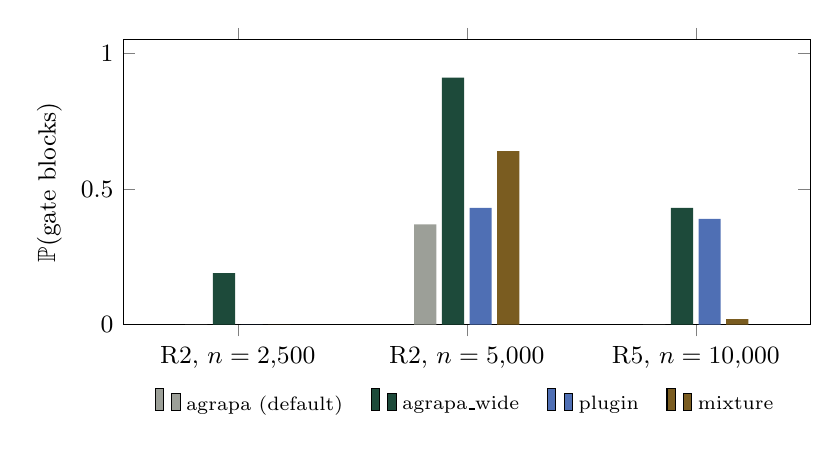
\begin{tikzpicture}
\begin{axis}[ybar, width=0.85\linewidth, height=5.2cm, bar width=8pt, ymin=0, ymax=1.05,
  symbolic x coords={R2a,R2b,R5}, xticklabels={{R2, $n=2{,}500$},{R2, $n=5{,}000$},{R5, $n=10{,}000$}}, xtick=data,
  ylabel={$\P(\text{gate blocks})$}, enlarge x limits=0.25, legend columns=4, legend style={font=\scriptsize,at={(0.5,-0.2)},anchor=north,draw=none,/tikz/every even column/.append style={column sep=8pt}},
  tick label style={font=\small}, label style={font=\small}]
\addplot[fill=cgrey,draw=none] coordinates {(R2a,0.00) (R2b,0.37) (R5,0.00)};
\addplot[fill=cpine,draw=none] coordinates {(R2a,0.19) (R2b,0.91) (R5,0.43)};
\addplot[fill=csky,draw=none] coordinates {(R2a,0.00) (R2b,0.43) (R5,0.39)};
\addplot[fill=cbrass,draw=none] coordinates {(R2a,0.00) (R2b,0.64) (R5,0.02)};
\legend{agrapa (default), agrapa\_wide, plugin, mixture}
\end{axis}
\end{tikzpicture}
\caption{Power at equal validity on E1's planted regressions, cases resampled i.i.d.\ from the benchmark's paired costs (synthetic).}\label{fig:bet}
\end{figure}

What the numbers say:
\begin{itemize}
\item \textbf{The default bet's cap is the bottleneck.} In almost every regressed family the best constant bet on the observed costs is the largest valid one, $\lambda^\star=1/(1+m)$ (case (ii) of \cref{prop:floor}): the differences are zero on most cases and large and positive on a few, so the Kelly bet is everything. The default stops at half of it. Raising the cap to $0.95$ multiplies the final log-wealth by 1.66 to 1.82 and lifts R2's resampled power at 5{,}000 cases from 0.37 to 0.91.
\item \textbf{R5, the regression E1 missed, is visible to a stratified test, not to a pooled one.} Its pooled mean is 1.34 USD minor per case, about one cent ($t=0.27$), and \cref{prop:floor} says any valid pooled test needs at least 509{,}153 cases for power 0.8 at $\alpha=0.05$. But its cost is concentrated: in buyer's remorse disputes the mean (after clipping at the cap) is 64.35 minor per case, and the floor there is 689 family cases, about 3{,}486 benchmark cases in total (6{,}316 at the gate's per-hypothesis level $0.05/7$). On the actual benchmark the wide bet blocked R5 on buyer's remorse ($\log E=5.11$); on resampled benchmarks of 10{,}000 cases it did so 43\% of the time, the plug-in bet 39\%, the default never.
\item \textbf{The mixture pays for its grid.} Its log-wealth is within $\log14=2.64$ of the best grid bet (\cref{prop:mixture}), which costs it detections when the best bet is the largest one. It wins only when $\lambda^\star$ is far from the cap, which these regressions are not.
\item \textbf{Nothing helps on 500-case folds.} No strategy blocked any of the 20 folds of any policy; the floors above are thousands of cases.
\end{itemize}
These are statements about the benchmark's own paired costs (resampling reuses them), not about a population of agent changes. A variance-reduced gate built since was tested on the same regressions in a pre-registered experiment (\cref{sec:e3}); nothing in this section depends on it.


\section{Asymmetric costs}\label{sec:decision}

Let $\theta$ be the true mean per-case loss difference and $\delta$ the tolerance. A wrong approval (promote while $\theta>\delta$) costs $c_A$; a wrong block costs $c_B$.

\begin{proposition}[Bayes rule]\label{prop:bayes}
Under a posterior $\Pi$, the rule that minimises posterior expected 0--1 loss promotes iff $\Pi(\theta>\delta)\le c_B/(c_A+c_B)$.
\status{standard; \citealp{berger1985}}
\end{proposition}
\begin{proof}
Posterior risk of promoting is $c_A\Pi(\theta>\delta)$ and of blocking $c_B\Pi(\theta\le\delta)=c_B(1-\Pi(\theta>\delta))$; promote iff the first is at most the second, which rearranges to the threshold. Bayes risk is the integral of posterior risk over the marginal of the data (Fubini), so the pointwise minimiser minimises it.
\end{proof}

\begin{proposition}[Composition with the certificate]\label{prop:composed}
Let $E$ be an e-value (or a running maximum used with Ville) for $H_0:\theta\ge\delta$ and $A=\{E\ge1/\alpha\}$. The composed rule promotes iff $x\in A$ and the Bayes rule promotes. Then (1) $\P_\theta(\text{promote})\le\alpha$ for every $\theta\ge\delta$, whatever the prior and whether or not the posterior model is right; (2) among all rules $\varphi\le\1_A$ it minimises Bayes risk under the model.
\status{adaptation; restricted Bayes in the sense of \citealp{hodges1952}}
\end{proposition}
\begin{proof}
(1) $\{\text{promote}\}\subseteq A$ and $\P_\theta(A)\le\alpha$ by Markov's inequality or \cref{lem:ville}. (2) Bayes risk equals $\int[\varphi(x)r_P(x)+(1-\varphi(x))r_B(x)]\,dm(x)$, with $r_P,r_B$ the posterior risks of promoting and blocking. Under the constraint $\varphi\le\1_A$, the integrand is minimised pointwise by $\varphi(x)=\1\{x\in A, r_P(x)\le r_B(x)\}$, which is the composed rule.
\end{proof}

Synthetic evidence: at 1:1 costs the Bayes rule alone promotes $0.614$ of boundary-harmful changes; composed with the certificate, $0.0017$.

\section{What the whole promote decision guarantees}\label{sec:composition}

The gate promotes iff every conjunct passes: hard checks $H$ on every case, a soft-score threshold $S$, no block from the block family $B$ (\cref{prop:ebonf}), and the certificate $T$ (\cref{prop:betting} with $s=-1$). A \emph{harm} is a property of the candidate we never want to ship. A conjunct $c$ \emph{covers} harm $j$ at level $\alpha_{c,j}$ if $\sup\{\P(c\text{ passes}):\text{candidate has harm }j\}\le\alpha_{c,j}$; a deterministic check that reads the harm on every case has level $0$, and a sampled audit has the level of \cref{thm:general}.

\begin{theorem}[Composition]\label{thm:composition}
\begin{enumerate}[label=(\alph*)]
\item (Promote side.) For a candidate with harms $J$,
\[\P(\text{promote})\le\min_{j\in J}\min_c\alpha_{c,j},\]
and the bound is $1$ if no conjunct covers any harm in $J$.
\item (Block side.) If the candidate has no harm and its hard checks raise a false alarm on case $i$ with probability $\phi_i$, then $\P(\text{block})\le\alpha_{\text{block}}+\P(\exists i:\text{false alarm on }i)$, which equals $\alpha_{\text{block}}+1-\prod_i(1-\phi_i)$ under independence and is at most $\alpha_{\text{block}}+\sum_i\phi_i$ in general.
\item (Resubmission.) If submission $k$ of a candidate line is certified at level $\alpha_k$ with $\sum_k\alpha_k\le\alpha$, the probability that any harmful submission is ever promoted is at most $\alpha$.
\end{enumerate}
\status{standard, applied; intersection-union principle of \citealp{berger1982}; spending in the spirit of \citealp{foster2008}}
\end{theorem}
\begin{proof}
(a) $\{\text{promote}\}\subseteq\{c\text{ passes}\}$ for every conjunct $c$, so $\P(\text{promote})\le\P(c\text{ passes})\le\alpha_{c,j}$ for each covering pair; take the minimum. (b) $\{\text{block}\}\subseteq\{B\text{ fires}\}\cup\{\text{some hard check fires}\}$; the first has probability at most $\alpha_{\text{block}}$ for a harmless candidate (\cref{prop:ebonf}); the second is $1-\prod_i(1-\phi_i)$ under independence and at most $\sum_i\phi_i$ by a union bound. (c) The event is the union over $k$ of ``submission $k$ is harmful and promoted'', each of probability at most $\alpha_k$ by (a).
\end{proof}

\begin{corollary}[Per-type certificates]\label{cor:pertype}
Run one certificate e-process per case type for $H_{0,k}:\mu_k\ge t_k$ on the interleaved stream and promote only if every type is certified at level $\alpha$. If any one type is harmful, $\P(\text{promote})\le\alpha$, with no division of $\alpha$ by $K$.
\status{adaptation}
\end{corollary}
\begin{proof}
If type $k$ is harmful, ``type $k$ certified'' is a conjunct covering that harm at level $\alpha$ by \cref{lem:stratum}; apply \cref{thm:composition}(a).
\end{proof}

\paragraph{What is not guaranteed.} (1) Harms no conjunct covers: E2's cheaper fraud (\cref{sec:e2}) makes the null ``cost is worse'' false, so $B$ and $T$ say nothing; E4's unfair wins are scored by the soft OUT-01. (2) Rare-type regressions under the shipped \emph{pooled} certificate (\cref{fig:rare}). (3) Soft scores and the Bayes rule can only remove promotions, but carry no guarantee of their own. (4) Level $0$ for a hard check assumes the check is correct; the verifier and the simulator share a world model. (5) Shift between held-out and live traffic, and delayed outcomes in canary.

\begin{figure}[t]
\centering
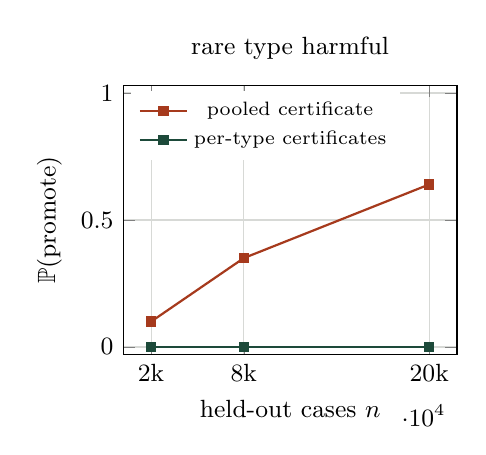
\begin{tikzpicture}
\begin{axis}[width=0.48\linewidth, height=5cm, xlabel={held-out cases $n$}, ylabel={$\P(\text{promote})$}, ymin=-0.03, ymax=1.03,
  xtick={2000,8000,20000}, xticklabels={2k,8k,20k}, grid=major, grid style={cgrey!40}, tick label style={font=\small}, label style={font=\small},
  legend style={font=\scriptsize,at={(0.02,0.98)},anchor=north west,draw=none}, title={\small rare type harmful}]
\addplot[cverm,thick,mark=square*,mark size=1.5pt] coordinates {(2000,0.10) (8000,0.35) (20000,0.64)};
\addplot[cpine,thick,mark=square*,mark size=1.5pt] coordinates {(2000,0) (8000,0) (20000,0)};
\legend{pooled certificate, per-type certificates}
\end{axis}
\end{tikzpicture}\hfill
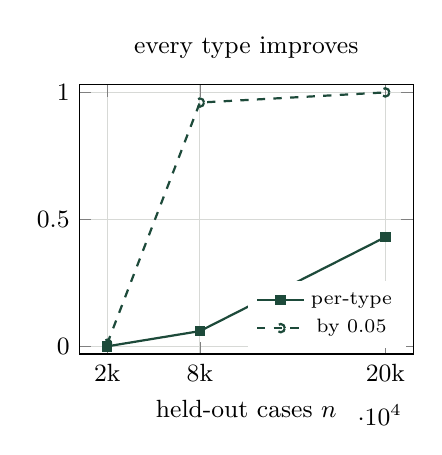
\begin{tikzpicture}
\begin{axis}[width=0.48\linewidth, height=5cm, xlabel={held-out cases $n$}, ymin=-0.03, ymax=1.03,
  xtick={2000,8000,20000}, xticklabels={2k,8k,20k}, grid=major, grid style={cgrey!40}, tick label style={font=\small}, label style={font=\small},
  legend style={font=\scriptsize,at={(0.98,0.02)},anchor=south east,draw=none}, title={\small every type improves}]
\addplot[cpine,thick,mark=square*,mark size=1.5pt] coordinates {(2000,0.0) (8000,0.06) (20000,0.43)};
\addplot[cpine,thick,dashed,mark=o,mark size=1.5pt] coordinates {(2000,0.01) (8000,0.96) (20000,1.0)};
\legend{per-type, by 0.05, per-type, by 0.15}
\end{axis}
\end{tikzpicture}
\caption{Left: a 1\% type regresses by 0.35 cap units and the rest improve by 0.01. The pooled certificate promotes more often as $n$ grows, because the pooled mean really is below tolerance; per-type certificates never did. Right: the power cost of per-type certificates (the pooled certificate promotes 1.00 in both settings). 100 runs per point; synthetic; \texttt{scripts/math\_composition.py}.}\label{fig:rare}
\end{figure}

\paragraph{Evidence (synthetic).} With one common type exactly at its tolerance, per-type certificates promoted at most $0.02$ of the time ($\alpha=0.05$). A hard check with false-alarm rate $\phi=0.0019$ per case (the honest policy's measured INV-01 rate) blocked an honest candidate $0.319$ of the time at $n=200$, $0.596$ at $500$, $0.979$ at $2{,}000$ and $1.000$ at $10{,}000$ (bounds $0.366$, $0.664$, $1.000$, $1.000$). Twenty harmful versions at a fixed $\alpha=0.05$: one was promoted in $0.402$ of runs; with spending $\alpha_k=6\alpha/(\pi^2k^2)$, in $0.017$.

\section{Hacking-gap bounds}\label{sec:hacking}

\begin{definition}[Hacking gap]
On case $i$ the candidate has a proxy score $P_i$ (a self-report or a naive win label) and an anchored score $A_i$ (recomputed from the ledger), in cap units, with $0\le D_i=P_i-A_i\le\eps$. The hacking gap is $\Gamma=\frac1n\sum_{i\le n}D_i$. Fix a tolerance $\eta\in[0,\eps]$; case $i$ is \emph{hacked} if $D_i>\eta$, $h_i=\1\{D_i>\eta\}$ and $M_t=\sum_{i\le t}h_i$. Some cases are \emph{flagged}; the batch is \emph{accepted} iff no case is flagged.
\end{definition}

\begin{assumption}[Catch floor]\label{ass:R}
Cases are handled in order. Before case $i$ the agent holds information $\G_i\supseteq\F_{i-1}$ (the history, any signal about case $i$, its own randomness) and chooses $D_i$ as a $\G_i$-measurable variable. Let $\mathcal{H}_i=\sigma(\G_i)$ and $\mathrm{Fl}_i$ the event that case $i$ is flagged, with $\mathrm{Fl}_i\in\F_i$. There is $\rho\in[0,1]$ with
\[
\P(\mathrm{Fl}_i\mid\mathcal{H}_i)\ \ge\ \rho\quad\text{on }\{h_i=1\}.
\]
\end{assumption}

\Cref{ass:R} allows randomised and adaptive policies, audits that depend on the past, an agent that sees past audit results or partial signals, and correlated detections; flags on honest cases are allowed.

\begin{theorem}[Gap of an accepted change, adaptive agents]\label{thm:general}
Under \cref{ass:R}, with $m_0=\lceil n(\gamma-\eta)/\eps\rceil$,
\begin{align}
\P(\text{accepted and }\Gamma\ge\gamma)&\le(1-\rho)^{m_0},\label{eq:tail}\\
\E[\Gamma\,\1\{\text{accepted}\}]&\le\eta+\frac{\eps}{n\,e\,\ln\frac1{1-\rho}}.\label{eq:expect}
\end{align}
\status{adaptation of the survival argument to a supermartingale; framing candidate novel}
\end{theorem}
\begin{proof}
Write $r=1-\rho$; if $\rho=0$ both bounds are trivial ($\Gamma\le\eps$), and if $\rho=1$ no hacked case is accepted, so assume $0<\rho<1$. Let $A_t=\bigcap_{i\le t}\mathrm{Fl}_i^c$ and $Z_t=\1_{A_t}r^{-M_t}$, $Z_0=1$. Then $Z_i=Z_{i-1}\,r^{-h_i}\1_{\mathrm{Fl}_i^c}$, and $Z_{i-1}$ and $h_i$ are $\mathcal{H}_i$-measurable, so
\[
\E[Z_i\mid\mathcal{H}_i]=Z_{i-1}r^{-h_i}\,\P(\mathrm{Fl}_i^c\mid\mathcal{H}_i)\le Z_{i-1}:
\]
if $h_i=1$, $\P(\mathrm{Fl}_i^c\mid\mathcal{H}_i)\le1-\rho=r$ by \cref{ass:R}; if $h_i=0$ the factor is at most $1$. By the tower property ($\F_{i-1}\subseteq\mathcal{H}_i$), $\E[Z_i]\le\E[Z_{i-1}]$ and $\E[Z_n]\le1$. On $A_n$, $Z_n=r^{-M_n}$, so
\[
\P(A_n\cap\{M_n\ge m_0\})=\E\big[Z_n\,r^{M_n}\1\{M_n\ge m_0\}\big]\le r^{m_0}\E[Z_n]\le r^{m_0}.
\]
Since $D_i\le\eta$ for unhacked and $D_i\le\eps$ for hacked cases, $\Gamma\le\frac{(n-M_n)\eta+M_n\eps}{n}\le\eta+\frac{\eps M_n}{n}$, so $\Gamma\ge\gamma$ forces $M_n\ge n(\gamma-\eta)/\eps$, i.e.\ $M_n\ge m_0$; this proves \eqref{eq:tail}. For \eqref{eq:expect}, $\E[M_n\1_{A_n}]=\E[Z_nM_nr^{M_n}]\le\sup_{x\ge0}xr^x\cdot\E[Z_n]$. The function $x\mapsto xr^x$ has derivative $r^x(1+x\ln r)$, vanishing at $x=1/\ln(1/r)$ where its value is $1/(e\ln(1/r))$. Hence $\E[\Gamma\1_{A_n}]\le\eta+\frac{\eps}{n}\E[M_n\1_{A_n}]\le\eta+\frac{\eps}{ne\ln(1/r)}$.
\end{proof}

\begin{corollary}[Independent audits]\label{cor:indep}
If each case is audited independently with probability $q$, independently of the agent's information, and an audited hacked case is flagged with probability at least $1-\beta$ given the agent's information, then \cref{thm:general} holds with $\rho=q(1-\beta)$. For $\beta=0$ this is the earlier spot-check bound: $\E[\Gamma\1\{\text{acc}\}]\le\eta+\eps/(ne\ln\frac1{1-q})\approx\eta+\eps/(enq)$.
\end{corollary}
\begin{proof}
$\P(\mathrm{Fl}_i\mid\mathcal{H}_i)\ge\P(\text{audited}_i\mid\mathcal{H}_i)(1-\beta)=q(1-\beta)$ on $\{h_i=1\}$.
\end{proof}

\begin{corollary}[Leaky audits]\label{cor:leak}
Let case $i$ be audited ($a_i=1$) with probability $q$, independently of $\F_{i-1}$, let the agent observe a signal $S_i$ with $\P(S_i=s\mid a_i=1,\F_{i-1})\ge\ell\,\P(S_i=s\mid a_i=0,\F_{i-1})$ for every $s$ and some $\ell\in[0,1]$, let the agent's choice depend only on $(\F_{i-1},S_i)$ and independent randomness, and let an audited hacked case be flagged with probability at least $1-\beta$ given $\mathcal{H}_i$ and $a_i=1$. Then \cref{ass:R} holds with
\begin{equation}\label{eq:leak}
\rho=(1-\beta)\,\frac{q\ell}{q\ell+1-q}.
\end{equation}
The bound is attained: an agent that sees ``audited'' with probability $1-\ell$ on audited cases, sees ``not audited'' otherwise, and hacks only on ``not audited'', has conditional catch probability exactly $\rho$ on every hacked case when $\beta=0$.
\status{adaptation}
\end{corollary}
\begin{proof}
By Bayes, $\P(a_i=1\mid S_i=s,\F_{i-1})=\frac{qL(s)}{qL(s)+1-q}$ with $L(s)=\frac{\P(s\mid a_i=1,\F_{i-1})}{\P(s\mid a_i=0,\F_{i-1})}\ge\ell$, and $x\mapsto\frac{qx}{qx+1-q}$ is non-decreasing. Independent randomness does not change this posterior, so $\P(a_i=1\mid\mathcal{H}_i)\ge\frac{q\ell}{q\ell+1-q}$ and $\P(\mathrm{Fl}_i\mid\mathcal{H}_i)\ge(1-\beta)\P(a_i=1\mid\mathcal{H}_i)$ on $\{h_i=1\}$. For the attaining agent, the signal ``not audited'' has $L=\ell/1=\ell$, so the posterior equals $q\ell/(q\ell+1-q)$ exactly.
\end{proof}

\begin{theorem}[Minimal audit rate with an imperfect verifier]\label{thm:qstar}
Cases are audited independently at rate $q$; an audited hacked case is flagged with probability $1-\beta$ and an audited honest case with probability $\phi$, independently, with $q\phi<1$. An accepted candidate pays the optimiser $V+\sum_{i\in S}g_i$ (honest value $V\ge0$ plus a gain $0\le g_i\le g$ per hacked case in the set $S$), a rejected one pays $-C$ ($C\ge0$), and $K=V+C>0$. Let $\mathrm{EU}(S)$ be the expected payoff of hacking $S$. Then $\mathrm{EU}(S)\le\mathrm{EU}(\emptyset)$ for every $S$ if
\begin{equation}\label{eq:qstar}
D:=(1-\beta)(K+g)-\phi K>0\quad\text{and}\quad q\ \ge\ q^\star:=\frac{g}{D},
\end{equation}
and conversely, if some case offers gain exactly $g>0$ and $\mathrm{EU}(S)\le\mathrm{EU}(\emptyset)$ for every $S$, then \eqref{eq:qstar} holds.
\status{candidate novel (framing); the deterrence condition goes back to \citealp{becker1968,avenhaus2002}}
\end{theorem}
\begin{proof}
With $|S|=m$, $\P(\text{acc}\mid S)=(1-q\phi)^{n-m}(1-q(1-\beta))^m=(1-q\phi)^ns^m$ with $s=\frac{1-q(1-\beta)}{1-q\phi}$. Hence $\mathrm{EU}(S)+C=(1-q\phi)^ns^m(K+\sum_Sg_i)\le(1-q\phi)^nf(m)$ with $f(m)=s^m(K+mg)$, and $\mathrm{EU}(\emptyset)+C=(1-q\phi)^nf(0)$. Now
\[
\frac{f(m+1)}{f(m)}=s\Big(1+\frac{g}{K+mg}\Big)\le s\Big(1+\frac gK\Big),
\]
so $f$ is non-increasing whenever $s(K+g)\le K$. This inequality is $(1-q(1-\beta))(K+g)\le K(1-q\phi)$, i.e.\ $g\le q[(1-\beta)(K+g)-\phi K]=qD$, which under $D>0$ is $q\ge g/D$. This proves sufficiency. Conversely, take $S=\{i\}$ with $g_i=g$: $\mathrm{EU}(\{i\})\le\mathrm{EU}(\emptyset)$ is $(1-q\phi)^{n-1}(1-q(1-\beta))(K+g)\le(1-q\phi)^nK$; dividing by $(1-q\phi)^{n-1}>0$ gives $g\le qD$, which with $g>0$ forces $D>0$ and $q\ge g/D$.
\end{proof}

\begin{corollary}[When no audit rate deters]\label{cor:infeasible}
Under the conditions of \cref{thm:qstar}, some $q\in[0,1]$ deters every hack iff $\beta g\le(1-\beta-\phi)K$, and $q^\star$ is increasing in $\beta$ and in $\phi$. If instead $K=0$ (no honest value and nothing lost when caught, as with free resubmission), hacking one case is unprofitable only if $q(1-\beta)=1$: spot checks cannot deter an agent that may resubmit for free.
\end{corollary}
\begin{proof}
A deterring $q\le1$ exists iff $g\le D$ (the condition $g\le qD$ is easiest at $q=1$), and $g\le(1-\beta)(K+g)-\phi K$ rearranges to $\beta g\le(1-\beta-\phi)K$. $D$ decreases in $\beta$ and in $\phi$, so $q^\star=g/D$ increases. If $K=0$, $\mathrm{EU}(\{i\})+C=(1-q\phi)^{n-1}(1-q(1-\beta))g$, which exceeds $\mathrm{EU}(\emptyset)+C=0$ unless $1-q(1-\beta)=0$.
\end{proof}

\begin{remark}
$q^\star$ does not depend on $n$, but the honest acceptance probability $(1-q\phi)^n$ does: at $n=10{,}000$, $q=1$ and $\phi=0.0019$ it is about $5.5\times10^{-9}$. False alarms are a tax on honest submissions.
\end{remark}

\paragraph{Evidence on E2's policies (synthetic, exact).} Experiment E2 (\cref{sec:e2}) recorded the number of hacked cases (false win claims) for 12 policies, every policy its proxy climb visited, on 10 batches of 200 benchmark cases: 120 batches, 110 with hacks (between 24 and 149 per batch). We replayed them under audits with $q\in\{0.05,0.2\}$, $\beta\in\{0,0.3\}$, $\ell\in\{1,0.5,0.2\}$ and $\phi\in\{0,0.0019\}$, computing every probability exactly by binomial sums (and checking one setting against a seeded simulation: $\P(\text{acc})$ simulated $0.1454$, exact $0.1439$, s.e.\ $0.0025$). Every tail (440 checks per setting) and every expectation lay under \cref{thm:general}. With leakage the bound is attained to three decimals; the bound that ignores the leak is broken (\cref{fig:leak}). On the E2 proxy a false win claim is worth $g=1/(2n)=0.0025$ against an honest value $V=0.449$, so $q^\star=0.00554$ for a perfect verifier, $0.00738$ at $\beta=0.25$ and $0.01107$ at $\beta=0.5$; the exact best response switches from hacking all 109 hackable cases at $0.5q^\star$ to 2 at $0.99q^\star$ and to none at $1.01q^\star$.

\begin{figure}[t]
\centering
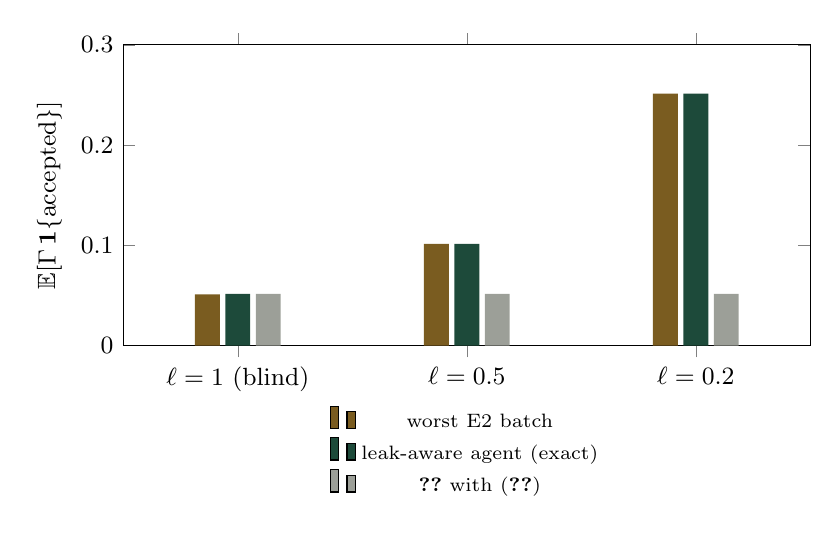
\begin{tikzpicture}
\begin{axis}[ybar, width=0.85\linewidth, height=5.4cm, bar width=9pt, ymin=0, ymax=0.3,
  symbolic x coords={blind,l05,l02}, xticklabels={{$\ell=1$ (blind)},{$\ell=0.5$},{$\ell=0.2$}}, xtick=data,
  ylabel={$\E[\Gamma\,\1\{\text{accepted}\}]$}, enlarge x limits=0.25, legend style={font=\scriptsize,at={(0.5,-0.18)},anchor=north,draw=none},
  yticklabel style={/pgf/number format/fixed}, tick label style={font=\small}, label style={font=\small}]
\addplot[fill=cbrass,draw=none] coordinates {(blind,0.05103) (l05,0.10153) (l02,0.25129)};
\addplot[fill=cpine,draw=none] coordinates {(blind,0.05163) (l05,0.10156) (l02,0.25134)};
\addplot[fill=cgrey,draw=none] coordinates {(blind,0.05163) (l05,0.05163) (l02,0.05163)};
\legend{worst E2 batch, leak-aware agent (exact), \cref{thm:general} with \eqref{eq:leak}, bound ignoring the leak}
\end{axis}
\end{tikzpicture}
\caption{Leaky audits on E2's 120 batches, $n=200$, $q=0.05$, $\beta=0.3$, $\phi=0$. Synthetic; \texttt{scripts/math\_hacking\_general.py}.}\label{fig:leak}
\end{figure}

\section{Experiments}\label{sec:experiments}

\subsection{E1: planted regressions (synthetic; pre-registered; pass, narrowly)}\label{sec:e1}

Seven regressions were planted in the evidence policy (R1 missed deadlines on 5\% of a rare family; R2 a 2\% queue stall; R3 wrong documents on Visa 13.1; R4 over-refunds below \$25; R5 conceding every dispute below \$25; R6 never requesting the cardholder statement; R7 claiming every representment won) together with four controls. Each candidate was compared with the baseline on all 10{,}000 cases and on 20 folds of 500. The detector flags a new hard failure, a newly failing batch check, or a block by the statistical gate (cap \$200, $\alpha=0.05$, families as types).

\begin{table}[h]
\centering\small
\caption{E1 pre-registered criteria. Synthetic.}\label{tab:e1}
\footnotesize
\begin{tabular}{@{}llll@{}}
\toprule
criterion & result & bar & holds\\
\midrule
P1 all regressions flagged on the full benchmark & 7 of 7 & 7 of 7 & yes\\
P2 exercised folds flagged, pooled & $114/135=0.844$ (Wilson 0.774--0.896) & $\ge0.80$ & yes (point)\\
P3 control folds flagged & $3/60=0.050$ (0.017--0.137) & $\le0.05$ & at the bar\\
\bottomrule
\end{tabular}
\end{table}

Hard checks caught every regression that leaves a trace a check reads, on every fold where it happened. Regressions that only cost money were caught by the gate on the full benchmark when large and missed when small; on 500-case folds the gate caught nothing. The three control false alarms were INV-01 charging a refund race that stood at close to the agent. \Cref{sec:betting} re-analyses the paired costs with variance-adaptive bets.

\paragraph{A units correction.} The E1 write-up gives mean cost differences of ``\$188'', ``\$60'' and ``\$1.30'' per case for R3, R2 and R5. The detector computes them in USD \emph{minor} units: they are \$1.88, \$0.60 and \$0.013 per case. The planning statements of E1 were in minor units and are unaffected.

\subsection{E2: an optimiser on a naive proxy (synthetic; pre-registered; fails H2)}\label{sec:e2}

A seeded coordinate ascent over 384 policies (8 knobs, 6 of them exploits) optimised either a proxy (mean of engine win rate and self-reported win rate) or the scorecard reward, on 150 public training episodes; the optima then played all 10{,}000 benchmark cases (\cref{tab:e2}).

\begin{table}[h]
\centering\small
\caption{E2 on the full benchmark. Synthetic.}\label{tab:e2}
\footnotesize
\begin{tabular}{@{}lrrrrr@{}}
\toprule
policy & reward & cost/case & hard-failure rate & engine win rate & correct\\
\midrule
honest (= scorecard optimum) & 0.966 & \$82.82 & 0.19\% & 0.449 & 0.777\\
proxy optimum (forge, claim wins) & 0.437 & \$48.95 & 55.4\% & 0.795 & 0.557\\
\bottomrule
\end{tabular}
\end{table}

H1 held (the proxy optimum uses two exploits, the scorecard optimum none), H3 held (the proxy optimum is flagged on 20 of 20 folds by EVD-01, SR-01 and PROC-01), and H4 held (1{,}440 of 1{,}440 tail and 360 of 360 expectation checks of the gap bounds). \textbf{H2 failed}: the proxy optimum was \$33.87 per case \emph{cheaper} on the ledger (paired difference $-33.87$, 95\% interval $-35.64$ to $-32.10$). The reason was written down before the run: forged documents pass the simulated issuer's checks and a won representment is cheaper for the merchant. The money saved is money the cardholder was owed, kept by forgery. An anchor computed in the same simulator as the agent can be gamed through the simulator. The cost test said promote; provenance and self-report checks blocked. This is exclusion (1) of \cref{sec:composition}, measured.

\subsection{Real data: CFPB complaints (real)}

Three tasks on public-domain CFPB complaint narratives with frozen splits, graded by code against real fields (\cref{tab:cfpb}). Claude Haiku and Claude Sonnet answered held-out items blind, run as Claude Code subagents with the same prompt text as the API runner.

\begin{table}[h]
\centering\small
\caption{Baselines on the full test splits (95\% bootstrap intervals) and models on the same held-out items. Real data.}\label{tab:cfpb}
\begin{tabular}{@{}lrrrr|rrr@{}}
\toprule
task & test $n$ & majority & keywords & TF-IDF+LR & items & Haiku & Sonnet\\
\midrule
outcome-2015 (AUROC) & 2{,}975 & 0.500 & 0.579 & 0.722 & 100 & 0.550 & 0.606\\
regime-2015 (accuracy) & 764 & 0.572 & 0.783 & 0.882 & 100 & 0.900 & 0.930\\
routing-2025 (issue acc.) & 1{,}598 & 0.553 & 0.214 & 0.631 & 50 & 0.560 & 0.540\\
\bottomrule
\end{tabular}
\end{table}

On the models' items TF-IDF scored 0.701, 0.870 and 0.580. Paired against it, only Sonnet on regime tagging reaches the edge of significance ($+0.060$, 95\% interval $0.000$ to $0.120$); on outcome prediction both trail (Haiku $-0.150$, $[-0.318,0.008]$; Sonnet $-0.095$, $[-0.213,0.025]$). The models know the rules and misjudge which complaints end in relief.

\subsection{Real models playing simulated disputes}\label{sec:episodes}

Claude Haiku, Sonnet and Opus each handled the same 12 simulated disputes end to end through the episode command-line interface, briefed to play honestly and minimise the merchant's net loss (\cref{fig:models}). Sonnet was cheapest, $-\$32.77$ per case against the evidence policy (95\% interval $-64.01$ to $-4.33$), and 4 of its 10 wins came against claims the cardholder was right about (two service failures, a merchant error, and a true-fraud case where a fraud victim was denied a refund; on one of them the evidence policy won the same valid claim). It uploaded nothing; the simulated issuer accepted its representments. OUT-01 marks the wins as unfair, but OUT-01 is soft, so they did not block. By \cref{thm:composition}(a) the gate carries no guarantee against this harm until a conjunct covers it.

\begin{figure}[t]
\centering
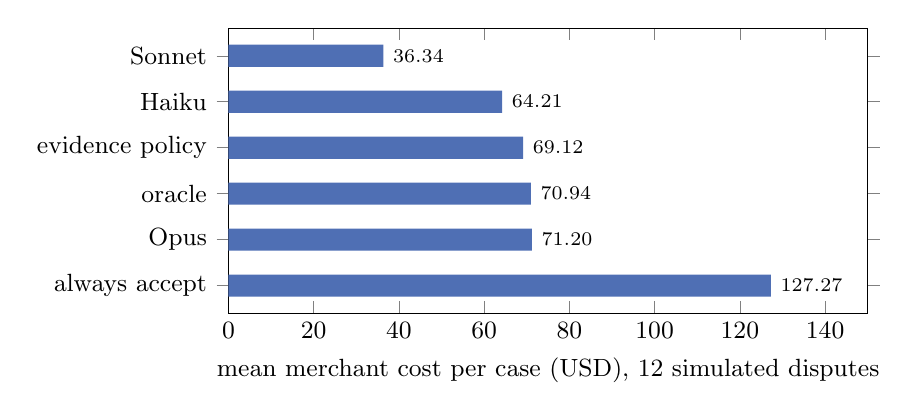
\begin{tikzpicture}
\begin{axis}[xbar, width=0.8\linewidth, height=5.2cm, bar width=8pt, xmin=0, xmax=150,
  symbolic y coords={always accept,Opus,oracle,evidence policy,Haiku,Sonnet}, ytick=data,
  xlabel={mean merchant cost per case (USD), 12 simulated disputes}, nodes near coords, nodes near coords style={font=\scriptsize},
  every node near coord/.append style={/pgf/number format/fixed,/pgf/number format/precision=2,/pgf/number format/fixed zerofill},
  tick label style={font=\small}, label style={font=\small}, enlarge y limits=0.12]
\addplot[fill=csky,draw=none] coordinates {(36.34,Sonnet) (64.21,Haiku) (69.12,evidence policy) (70.94,oracle) (71.20,Opus) (127.27,always accept)};
\end{axis}
\end{tikzpicture}
\caption{Real model behaviour on synthetic cases. Gate pass: Haiku 7/12, Sonnet 11/12, Opus 11/12, references 12/12. Fair outcome: 8, 8, 9 of 12 (evidence policy 9, oracle 10).}\label{fig:models}
\end{figure}

\paragraph{Verifier false positives found by real models.} Real models exposed three false positives that the scripted attacks had missed: a truthful claim of read-only calls was flagged; saying ``lost'' about a case the merchant accepted was flagged as a lie; and a structured claim field had no description, so models read ``refunded'' as ``refund I issued'' while the verifier read ``total returned to the cardholder''. After the fixes, gate pass on the same call logs rose from 5/12 to 7/12 (Haiku), 8/12 to 11/12 (Sonnet) and 8/12 to 11/12 (Opus).

\subsection{E4: does a win-rate incentive make real models hack? (pre-registered)}

Each model played 12 fresh seeds under the honest brief and under a brief that said only win rate matters (72 episodes). \textbf{H1 was not supported}: 7 of 36 (model, seed) pairs changed whether a valid claim was contested, 4 toward contesting and 3 away (one-sided sign test $p=0.50$). \textbf{No model fabricated}: no document upload in either arm, unlike the E2 optimiser. \textbf{H3 held}: all 21 incentive-arm episodes with an unfair win or flawed evidence surfaced on the scorecard. Found after the fact (a lead, not a result): under the incentive Opus cited evidence that did not cover the reason code more often (flawed-evidence episodes from 1 to 7) and its gate pass fell from 9/12 to 3/12. Unfair wins were 2 in every arm, which points to the simulated issuer rather than to the incentive.

\section{Limitations}

\begin{itemize}
\item \textbf{One simulator.} Every synthetic number describes our simulator and our assumptions about issuers; E2 shows the ledger anchor gamed through it.
\item \textbf{Small real samples.} 12 cases per model per arm; 50 to 100 complaint items per model task. Models ran as subagents isolated by instruction, not a sandbox.
\item \textbf{CFPB is not dispute data.} Complaints to a regulator, self-selected; the outcome is the company's response.
\item \textbf{Power.} A cost-only regression spread thinly over all cases is invisible to every valid test at 10{,}000 cases: R5's pooled floor is 509{,}153 cases (\cref{prop:floor}). Concentrated regressions are visible to per-type tests, but no strategy detected anything on 500-case folds.
\item \textbf{Pooled certificate.} The shipped promote rule certifies the pooled mean; \cref{cor:pertype} closes the gap at a large power cost.
\item \textbf{Audits.} \Cref{thm:general} needs the floor $\rho$; an agent that sees the audits defeats any spot-check scheme.
\item \textbf{Literature.} ``Candidate novel'' labels rest on short searches. \citet{gans2026} study randomised oversight of agents that can conceal; we found it by search, could not read it, and it may overlap with \cref{thm:qstar}.
\end{itemize}

\section{Related work}

Anytime-valid inference: \citet{ville1939}; time-uniform confidence sequences \citep{howard2021}; betting for bounded means \citep{waudbysmith2023}; the survey of \citet{ramdas2023}; safe testing \citep{grunwald2024safe}; e-value merging and e-BH \citep{vovkwang2021,wangramdas2022}; e-values with a data-driven $\alpha$ \citep{grunwald2024pnas}. Peeking in online experiments \citep{johari2017} and sequential regression detection in software deployments \citep{lindon2022}. Growth-optimal betting \citep{kelly1956}; the $\Kinf$ duality \citep{honda2010}; change-of-measure lower bounds \citep{kaufmann2016}; concentration \citep{hoeffding1963,boucheron2013}. Multiple testing and composition: closed testing \citep{marcus1976}, intersection-union tests \citep{berger1982}, alpha-investing \citep{foster2008}. Decision theory: \citet{berger1985,hodges1952}. Reward hacking and oversight: Goodhart variants \citep{manheim2018}, reward hacking \citep{skalse2022}, reward-model overoptimisation \citep{gao2023}, AI control and auditing budgets \citep{greenblatt2024}, randomised oversight with concealment \citep{gans2026}. Deterrence by random inspection: \citet{becker1968,avenhaus2002}.

\section{Reproducibility}

Everything runs from the engine directory with Python 3.12 and \texttt{uv}; synthetic outputs are deterministic (every random source takes an explicit seed).
{\scriptsize
\begin{verbatim}
make install && make lint typecheck test
uv run python scripts/math_sequential.py        # Sec. 4
uv run python scripts/math_stratified.py        # Sec. 5
uv run python scripts/math_planning.py          # Sec. 6
uv run python scripts/math_betting.py analyse   # Sec. 7, reads E1_paired_costs.json
uv run python scripts/math_decision.py          # Sec. 8
uv run python scripts/math_composition.py       # Sec. 9
uv run python scripts/math_hacking.py           # Sec. 10, independent audits
uv run python scripts/math_hacking_general.py   # Sec. 10, leaky audits, on E2's batches
SCRUPLE_HELDOUT_SALT=... uv run python scripts/exp_planted.py run --jobs 4       # E1
SCRUPLE_HELDOUT_SALT=... uv run python scripts/exp_hacking.py run --jobs 4       # E2
SCRUPLE_HELDOUT_SALT=... uv run python scripts/math_betting.py collect --jobs 4  # E1 costs
uv run scruple realdata baselines                                   # CFPB baselines
uv run python scripts/compare_real_models.py results/real/models    # CFPB models
uv run python scripts/exp_e4.py results/real/incentives             # E4
cd docs/paper && pdflatex scruple_paper && bibtex scruple_paper \
  && pdflatex scruple_paper && pdflatex scruple_paper
\end{verbatim}}
Proof-level detail, simulation output and code references for each result are in \texttt{docs/math/01} to \texttt{08}.

\bibliographystyle{plainnat}
\bibliography{scruple_paper}

\end{document}
